% Chapter 1

\chapter{Introduction} % Main chapter title

\label{Chapter1} % For referencing the chapter elsewhere, use \ref{Chapter1} 

%----------------------------------------------------------------------------------------

\section{User friendly Data analysis: gAn Web}

GAn is a program that aims to analyse huge amount of data related to the AEgIS experiment at the CERN.
 
This program receive in input a folder containing several terabytes of files in ".root" format, and parameter named "run parameter", that identifies the information in which the users are interested. 
A file ".root" is a file produced by a variegated group of sensors in a complex machine that accelerates particles and lets them crash together. This sensors produce .root files continuously (8 hours per day). The time in this experiment is divided in "runs" (a run lasts about 140 seconds), so the user, by the run parameter can tell to gAn in which time slice he is interested.

The .root files can be analysed using a framework named ROOT Framework, that consists in a lot of libraries specialized in high-energy physics analysis, and an interpreter able to understand a C++ script.
Actually, gAn is the sum of the Root Framework plus a lot of C++ scripts.
The goal of gAn is reduce the huge amount of raw data in input in a little amount of scientifically interesting data in output. To do this it has to filter data, understand which of them are scientifically interesting, chose the parts that are related to the run selected by the user (by the run parameter), elaborate and compare them, and make advanced statistical analysis on them.  
gAn can be called using a common linux terminal, using a command with parameters. 

The output of gAn consists of a single text file with computed, organized data, and a folder of images in png format. 
This structure (root files in input, data analysis using Root, images, organized and selected data in output) is very common in the CERN's experiments. 
The output of gAn is quite understandable by an experienced physicist, but it is disorganized, complex for an untrained user, and and the terminal interface can be surely improved using some more user friendly technologies.


GAn Web is a web application, that aims to create a user friendly web interface, based on the most important human-machine interaction principles, between the users and gAn.
A web interface can improve it in two ways:

\begin{enumerate}

% 1
\item gAn is a stand-alone program based on Root, installable on the user's machine; the user has to install the correct version of Root to avoid compatibility problems (Root is still not perfectly version independent: different versions can lead to different behaviours). Furthermore, this kind of program is continuously changing, the performed analysis is continuously improved, so the installed version of gAn is not final and unchangeable, and the user musts often update it. Instead, a centralized version installed on a server, with services accessible from a normal browser by the user can avoid (at least reduce) this kind of problems and be more usable.    
 

% 2
\item a Linux terminal interface is practical for expert users, but a web based interface can be more attractive for new users, and, if well done, can be easier to use. It is important to notice that the users are physicists, not necessarily specialized in computer science, so, create a friendly and easily learnable interface can avoid them problems and time wasting.   


\end{enumerate}


The goal of gAn Web is to allow users to do analysis through a more friendly web interface, without install nothing on their machine. In the following image there is a schema that shows how this program is organized.

\begin{figure}[H]
\centering
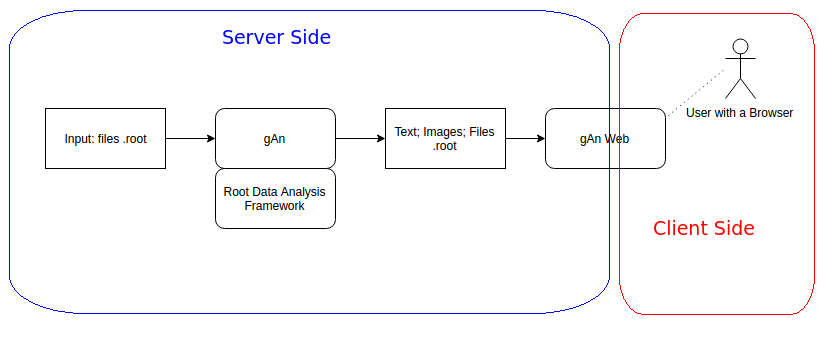
\includegraphics[scale=0.5]{GeneralGAnSchema.png} 
\caption{gAn - gAn Web simple scheme}
\end{figure}



